% Copyright (C) Data Structures and Algorithms Team.
\chapter{Linked Lists}
Linked lists can be thought of from a high level perspective as being a series of nodes, each node has at least a pointer to the next node, and in the last nodes case a null pointer representing that there are no more nodes to follow.
The general characteristics of linked lists are as follows:

\begin{enumerate}
\item Insertion is $O(1)$
\item Deletion is $O(n)$
\item Searching is $O(n)$
\end{enumerate}

Out of the three operations the one that stands out is that of insertion, in DSA we chose to always maintain pointers (or more aptly references) to the node(s) at the head and tail of the linked list and so performing a traditional insertion to either the front or back of the linked list is an $O(1)$ operation. An exception to this rule is when performing an insertion before a node that is neither the head nor tail in a singly linked list, that is the node we are inserting before is somewhere in the middle of the linked list. It is apparent that in order to add before the designated node we need to traverse the linked list to acquire a pointer to the node before the node we want to insert before which yields an $O(n)$ run time.

These data structure's are trivial, but they have a few key points which at times make them very attractive: 
\begin{enumerate}
\item the list is dynamically resized, thus it incurs no copy penalty like an array or vector would eventually incur; and
\item insertion is $O(1)$.
\end{enumerate}

\section{Singly Linked List}
Singly linked list's are one of the most primitive data structures you will find in this book, each node that makes up a singly linked list consists of a value, and a reference to the next node (if any) in the list. 

\begin{figure}
\caption{Singly linked list node}
\begin{center}
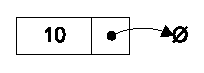
\includegraphics{singly_linked_list_node}
\end{center}
\end{figure}

\subsection{Insertion} \label{single_insertion}
In general when people talk about insertion with respect to linked lists of any form they implicitly refer to the adding of a node to the tail of the list, thus when you use an API like that of DSA and you see a general purpose method that adds a node to the list assume that you are adding that node to the tail of the list not the head.

Adding a node to a singly linked list has only two cases: 
\begin{enumerate}
\item $head = \emptyset$ in which case the node we are adding is now both the $head$ and $tail$ of the list; or
\item we simply need to append our node onto the end of the list updating the $tail$ reference appropriately.
\end{enumerate}

\begin{tabbing}
1)  \textbf{alg}\= \textbf{orithm} Add($value$) \\
2)  \> \textbf{Pre:}~~$value$ is the value to add to the list \\
3)  \> \textbf{Post:}~$value$ has been placed at the tail of the list \\
4)  \> $n \leftarrow$ node($value$) \\
5)  \> \textbf{if}~\= $head = \emptyset$ \\
6)  \> \> $head \leftarrow n$ \\
7)  \> \> $tail \leftarrow n$ \\
8)  \> \textbf{else} \\
9)  \> \> $tail$.Next $\leftarrow n$ \\
10) \> \> $tail \leftarrow n$ \\
11) \> \textbf{end if} \\
12) \textbf{end} Add \\
\end{tabbing}

As an example of the previous algorithm consider adding the following sequence of integers to the list: $1$, $45$, $60$, and $12$, the resulting list is that of Figure \ref{fig:singly_populated_list}.

\begin{figure}
\caption{A singly linked list populated with integers}
\label{fig:singly_populated_list}
\begin{center}
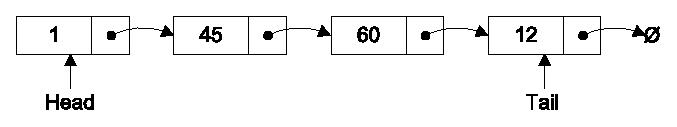
\includegraphics{singly_linked_list_populated_list}
\end{center}
\end{figure}

\subsection{Searching} \label{single_search}
Searching a linked list is straight forward, we simply traverse the list checking the value we are looking for with the value of each node in the linked list. The algorithm listed in this section is very similar to that used for traversal in \S\ref{singly_linked_traversal}.

\begin{tabbing}
1)  \textbf{alg}\= \textbf{orithm} Contains($head$, $value$) \\
2)  \> \textbf{Pre:}~~$head$ is the head node in the list \\
3)  \> ~~~~~~~~$value$ is the value to search for \\
4)  \> \textbf{Post:}~the item is either in the linked list, true; otherwise false \\
5)  \> $n \leftarrow head$ \\
6)  \> \textbf{whi}\= \textbf{le} $n~!= \emptyset$ \textbf{and} $n$.Value $!= value$ \\
7)  \> \> $n \leftarrow n$.Next \\
8)  \> \textbf{end while} \\
9)  \> \textbf{if} $n = \emptyset$ \\
10) \> \> \textbf{return false} \\
11) \> \textbf{else} \\
12) \> \> \textbf{return true} \\
13) \> \textbf{end if} \\
14) \textbf{end} Contains \\
\end{tabbing}

\subsection{Deletion} \label{single_deletion}
Deleting a node from a linked list is straight forward but there are a few cases in which we need to accommodate for:
\begin{enumerate}
\item the list is empty; or
\item the node to remove is the only node in the linked list; or 
\item we are removing the head node; or
\item we are removing the tail node; or
\item the node to remove is somewhere in between the head and tail; or
\item the item to remove doesn't exist in the linked list
\end{enumerate}

\begin{tabbing}
1)  \textbf{alg}\= \textbf{orithm} Remove($head$, $value$) \\
2)  \> \textbf{Pre:}~~$head$ is the head node in the list \\
3)  \> ~~~~~~~~$value$ is the value to remove from the list \\
4)  \> \textbf{Post:}~$value$ is removed from the list, true; otherwise false \\
5)  \> \textbf{if}~\= $head = \emptyset$ \\
6)  \> \> // case 1 \\
7)  \> \> \textbf{return false} \\
8)  \> \textbf{end if} \\
9)  \> $n \leftarrow head$ \\
10) \> \textbf{if} $n$.Value $= value$ \\
11) \> \> \textbf{if}~\= $n = head$ \textbf{and} $n = tail$ \\
12) \> \> \> // case 2 \\
13) \> \> \> $head \leftarrow \emptyset$ \\
14) \> \> \> $tail \leftarrow \emptyset$ \\
15) \> \> \textbf{else} \\
16) \> \> \> // case 3 \\
17) \> \> \> $head \leftarrow head$.Next \\
18) \> \> \textbf{end if} \\
19) \> \> \textbf{return true} \\
20) \> \textbf{end if} \\
21) \> \textbf{while} $n$.Next $!= \emptyset$ \textbf{and} $n$.Next.Value $!= value$ \\
22) \> \> $n \leftarrow n$.Next \\
23) \> \textbf{end while} \\
24) \> \textbf{if} $n$.Next $!= \emptyset$ \textbf{and} $n$.Next.Value $= value$ \\
25) \> \> \textbf{if} $n$.Next $= tail$ \\
26) \> \> \> // case 4 \\
27) \> \> \> $tail \leftarrow n$ \\
28) \> \> \textbf{end if} \\
29) \> \> // this is only case 5 if the conditional on line 25) was $ff$ \\
30) \> \> $n$.Next $\leftarrow n$.Next.Next \\
31) \> \> \textbf{return true} \\
32) \> \textbf{end if} \\
33) \> // case 6 \\
34) \> \textbf{return false} \\
35) \textbf{end} Remove \\
\end{tabbing}

\subsection{Traversing the list} \label{singly_linked_traversal}
Traversing a singly list is the same as that of traversing a doubly linked list, you start at the head of the list and continue until you come across a node that is $\emptyset$. The two cases are as follows:
\begin{enumerate}
\item $node = \emptyset$, we have exhausted all nodes in the linked list; or
\item we must update the $node$ reference to be $node$.Next.
\end{enumerate}

The algorithm described is a very simple one that makes use of a simple $while$ loop to check the first case.

\begin{tabbing}
1)  \textbf{alg}\= \textbf{orithm} Traverse($head$) \\
2)  \> \textbf{Pre:}~~$head$ is the head node in the list \\
3)  \> \textbf{Post:}~the items in the list have been traversed \\
4)  \> $n \leftarrow head$ \\
5)  \> \textbf{whi}\=\textbf{le} $n~!= 0$ \\
6)  \> \> \textbf{yield} $n$.Value \\
7)  \> \> $n \leftarrow n$.Next \\
8)  \> \textbf{end while} \\
9)  \textbf{end} Traverse \\
\end{tabbing}

\subsection{Traversing the list in reverse order}
Traversing a singly linked list in a forward manned is simple (i.e. left to right) as demonstrated in \S\ref{singly_linked_traversal}, however, what if for some reason we wanted to traverse the nodes in the linked list in reverse order? The algorithm to perform such a traversal is very simple, and just like demonstrated in \S\ref{single_deletion} we will need to acquire a reference to the previous node of a node, even though the fundamental characteristics of the nodes that make up a singly linked list prohibit this by design.

\begin{tabbing}
1)  \textbf{alg}\= \textbf{orithm} ReverseTraversal($tail$) \\
2)  \> \textbf{Pre:}~~$tail$ is the tail node in the list \\
3)  \> \textbf{Post:}~the items in the list have been traversed in reverse order \\
4)  \> \textbf{if}~\= $tail~!= \emptyset$ \\
5)  \> \> $curr \leftarrow tail$ \\
6)  \> \> \textbf{whi}\= \textbf{le} $curr~!= head$ \\
7)  \> \> \> $prev \leftarrow head$ \\
8)  \> \> \> \textbf{whi}\= \textbf{le} $prev$.Next $!= curr$ \\
9)  \> \> \> \> $prev \leftarrow prev$.Next \\
10) \> \> \> \textbf{end while} \\
11) \> \> \> \textbf{yield} $curr$.Value \\
12) \> \> \> $curr \leftarrow prev$ \\
13) \> \> \textbf{end while} \\
14) \> \> \textbf{yield} $curr$.Value \\
15) \> \textbf{end if} \\
16) \textbf{end} ReverseTraversal \\
\end{tabbing}

\section{Doubly Linked List}
Doubly linked lists are very similar to singly linked lists, the only difference is that each node has a reference to both the next and previous nodes in the list.

\begin{figure}
\caption{Doubly linked list node}
\begin{center}
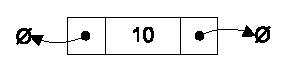
\includegraphics{doubly_linked_list_node}
\end{center}
\end{figure}


It would be wise to point out that the following algorithms for the doubly linked list are exactly the same as those listed previously for the singly linked list:

\begin{enumerate}
\item Searching (defined in \S\ref{single_search})
\item Traversal (defined in \S\ref{singly_linked_traversal})
\end{enumerate}

\subsection{Insertion}
The only major difference between the algorithm in \S\ref{single_insertion} is that we need to remember to bind the previous pointer of $n$ to the previous tail node if $n$ was not the first node to be inserted into the list.

\begin{tabbing}
1)  \textbf{alg}\= \textbf{orithm} Add($value$) \\
2)  \> \textbf{Pre:}~~$value$ is the value to add to the list \\
3)  \> \textbf{Post:}~$value$ has been placed at the tail of the list \\
4)  \> $n \leftarrow$ node($value$) \\
5)  \> \textbf{if}~\= $head = \emptyset$ \\
6)  \> \> $head \leftarrow n$ \\
7)  \> \> $tail \leftarrow n$ \\
8)  \> \textbf{else} \\
9)  \> \> $n$.Previous $\leftarrow tail$ \\
10) \> \> $tail$.Next $\leftarrow n$ \\
11) \> \> $tail \leftarrow n$ \\
12) \> \textbf{end if} \\
13) \textbf{end} Add \\
\end{tabbing}

Figure \ref{doubly_linked_list_add} shows the doubly linked list after adding the sequence of integers defined in \S\ref{single_insertion}.

\begin{figure}[h]
\caption{Doubly linked list populated with integers} \label{doubly_linked_list_add}
\begin{center}
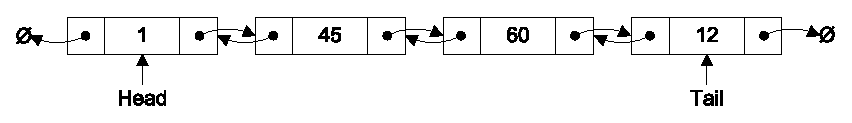
\includegraphics{doubly_linked_list_populated}
\end{center}
\end{figure}

\subsection{Deletion}
As you may of guessed the cases that we use for deletion in a doubly linked list are exactly the same as those defined in \S\ref{single_deletion}, however, like insertion we have the added task of binding an additional reference ($Previous$) to the correct value.

\newpage
\begin{tabbing}
1)  \textbf{alg}\= \textbf{orithm} Remove($head$, $value$) \\
2)  \> \textbf{Pre:}~~$head$ is the head node in the list \\
3)  \> ~~~~~~~~$value$ is the value to remove from the list \\
4)  \> \textbf{Post:}~$value$ is removed from the list, true; otherwise false \\
5)  \> \textbf{if}~\= $head = \emptyset$ \\
6)  \> \> \textbf{return false} \\
7)  \> \textbf{end if} \\
8)  \> \textbf{if} $value = head$.Value \\
9)  \> \> \textbf{if}~\= $head = tail$ \\
10) \> \> \> $head \leftarrow \emptyset$ \\
11) \> \> \> $tail \leftarrow \emptyset$ \\
12) \> \> \textbf{else} \\
13) \> \> \> $head \leftarrow head$.Next \\
14) \> \> \> $head$.Previous $\leftarrow \emptyset$ \\
15) \> \> \textbf{end if} \\
16) \> \> \textbf{return true} \\
17) \> \textbf{end if} \\
18) \> $n \leftarrow head$.Next \\
19) \> \textbf{while} $n~!= \emptyset$ \textbf{and} $value~!= n$.Value \\
20) \> \> $n \leftarrow n$.Next \\
21) \> \textbf{end while} \\
22) \> \textbf{if} $n = tail$ \\
23) \> \> $tail \leftarrow tail$.Previous \\
24) \> \> $tail$.Next $\leftarrow \emptyset$ \\
25) \> \> \textbf{return true} \\
26) \> \textbf{else if} $n~!= \emptyset$ \\
27) \> \> $n$.Previous.Next $\leftarrow n$.Next \\
28) \> \> $n$.Next.Previous $\leftarrow n$.Previous \\
29) \> \> \textbf{return true} \\
30) \> \textbf{end if} \\
31) \> \textbf{return false} \\
32) \textbf{end} Remove \\
\end{tabbing}
